\documentclass{article}

\usepackage{polski}
\usepackage[utf8]{inputenc}
\usepackage{amsmath}	
\usepackage{graphicx}
\usepackage{amsfonts}
\usepackage{hyperref}
\usepackage{tabstackengine}
\usepackage{caption}
\usepackage{subfig}

\newcommand{\bb}{\textbf}

\title{Praca inżynierska}
\date{2017-10-01}
\author{Jędrzej Kozal}

\begin{document}



\begin{titlepage}
	\centering
	
\includegraphics[width=0.25\textwidth]{logo_pol_wroclaw.png}\par\vspace{1cm}
	{\scshape\LARGE Politechnika Wrocławska \par}
	\vspace{1cm}
	{\scshape\Large Praca inżynierska\par}
	\vspace{1.5cm}
	{\huge\bfseries Biometryczny system kontroli dostępu - przetwarzanie obrazów i przygotowanie danych dla sieci neuronowych \par}
	\vspace{2cm}
	{\Large\itshape Jędrzej Kozal\par}
	\vfill
	promotor\par
	Dr inż.~Piotr \textsc{Ciskowski}

	\vfill

% Bottom of the page
	{\large 2017-10-01\par}
\end{titlepage}


\section{Wstęp}
Celem pracy jest porównanie metod i algorytmów umożliwiających wykrycie twarzy na zdjęciu, oraz wyznaczenie wektora uczącego dla sieci neuronowej na podstawie wyznaczonego zdjęcia twarzy. Projekt ten jest częścią systemu biometrycznej kontroli dostępu. Za implementację sieci neuronowych oraz analizę algorytmów związanych z sieciami odpowiadał Filip Guzy. Za architekturę systemu, oraz komunikację pomiędzy komponentami odpowiadał Michał Leś.
\subsection{Omówienie zagadnienia}

\subsection{Omawiany komponent jako część większego systemu}
\subsubsection{Wykorzystane wzorce projektowe}

W celu ułatwienia pracy współpracownikom w projekcie został utworzony wydzielony łatwo wymienialny komponent. W celu ułatwienia pracy badawczej komponent został podzielony na mniejsze elementy z wykorzystaniem obiektowych wzorców projektowych.
Do reprezentacji całego komponentu wybrano wzorzec fabryka. Zapewniono w ten sposób elastyczność użytkownikom klasy, ponieważ mogą oni zdecydować w jaki sposób współrzędne będące wynikiem działania algorytmów mają być przedstawione. Zapewniono klasę bazową do przechowywania współrzędnych, po której dziedziczą poszczególne reprezentacje, takie jak bezpośrednie przechowywanie danych w pamięci programu, czy zapis na pamięć nieulotną w postaci pliku z rozszerzeniem .npy z biblioteki numpy.
W celu zwiększenia elastyczności w obrębie komponentu do wyboru algorytmów dwukrotnie wykorzystano wzorzec strategia. Stworzono klasy bazowe do reprezentacji podstawowych własności algorytmu, które następnie implementowano w klasach pochodnych. Modyfikacja ta ułatwiła pracę badawczą i usystematyzowała strukturę projektu.
\subsubsection{Wykorzystane zasady i dobre praktyki programowania}

W trakcie realizacji projektu oprócz wykorzystania wzorców projektowych posługiwano się także dobrymi zasadami SOLID oraz clean code. Pozwalają one na zachowanie większego porządku oraz czytelności kodu. Dobra organizacja kodu oraz porządek ułatwiają rozwijanie projektu oraz systematyzują pracę. Nie zdecydowano się na wykorzystanie testów jednostkowych ze względu na dynamiczny charakter projektu. Definiowanie zachowań w testach jednostkowych jest kosztowne, a częste zmiany powodują że praca ta momentami byłaby zbędna.

\subsubsection{Wykorzystane biblioteki, narzędzia i zasoby}
Projekt systemu biometrycznej kontroli dostępu został zrealizowany całkowicie w języku programowania Python. Decyzja ta była podyktowana głównie znaczącą ilością gotowych bibliotek, które znacząco ułatwiają pracę. Wykorzystana została wersja języka 2.7.9, ponieważ biblioteki języka Python często wymagają wersji 2.7 lub wyższej. W omawianym komponencie wykorzystano biblioteki NumPy, SciPy, scikit-learn oraz openCV. 
NumPy to biblioteka zawierająca wiele algorytmów do realizacji obliczeń numerycznych oraz implementację wielu matematycznych narzędzi związanych z algebrą liniową. Implementacja algorytmów macierzowych z NumPy cieszy się dużą popularnością, dlatego warto poświęcić czas na poznanie tej biblioteki, ponieważ stanowi ona fundament wielu innych projektów i bibliotek.
SciPy jest biblioteką wykorzystywaną do obliczeń naukowych i inżynierskich. Zawiera algorytmy umożliwiające przeprowadzane obliczeń w wielu dziedzinach, dlatego również jest wykorzystywana jako baza innych projektów.
Instalacja SciPy jest prerekwizytem do instlacji scikit-learn. Scikit-learn to biblioteka zawierająca wiele algorytmów z dziedziny machine learning oraz pattern recognition. Jest to kluczowa bilioteka w omawianym projekcie, ponieważ dostarcza najistatniejszych narzędzi. Jej zastosowanie znacznie ułatwiło pracę.
OpenCv stanowi poteżny zbiór narzędzi do analizy oraz przetwarzania obrazów. Rozpowszechniana w ramach licencji . Twórcy biblioteki skupiają się na działanie w czasie rzeczywistym i zapewniają wielordzeniowe przetwarzanie. Jest to znaczące ułatwienie biorąc pod uwagę podstawową platformę sprzętową, na której był realizowany projekt. 

Wszystkie wymienione biblioteki są rozpowszechniane w ramach licencji new-BSD lub 3-clause BSD, co oznacza że wolno je wykorzystywać w celach akademickich lub komercyjnych. Zastosowanie bibliotek dostarczających zoptymalizowanych algorytmów znacznie ułatwiło i usystematyzowało pracę nad projektem.

Na początku pracy nad projektem podjęto próbę implementacji własnej wersji algorytmu PCA, aby lepiej zrozumieć i dokładnie prześledzić jego działanie. Algorytm ten działał poprawnie, ale względu na dużą złożoność obliczeniową zdecydowano się na korzystanie z wersji udostępnionej w bibliotece scikit-learn. W trakcie późniejszych prac nad systemem znaleziono informację na temat tego co powodowało tak wysoką złożoność obliczeniową oraz sposób na jej uniknięcie. Zagadnienie to zostało opisane w rozdziale Realizacja algorytmu.

Wykorzystane bazy zdjęć

\section{Implementacja algorytmów – detekcja twarzy}
 
\subsection{Przetwarzanie obrazu po akwizycji} 
 
 
 \newpage
 
\section{Implementacja algorytmów – ekstrakcja cech}

Pomiędzy tymi etapami obraz jest obcinany do rozmiaru 64 $\times$ 64, w celu zwiększenia szybkości przetwarzania.
 
\subsection{Principle Components Analysis}

Principle Components Analysis (PCA) jest algorytmem redukcji wymiarowości danych. Mając określony zbiór obserwacji, będący reprezentatywną reprezentacją próbą analizowanej przestrzeni należy wyznaczyć zbiór wektorów bazowych, tak aby wariancja danych z zbioru obserwacji względem nowo wyznaczownych wektorów bazowych była jak najwyższa.

\subsubsection{Wstęp matematyczny}

Przedstawione tutaj wyprowadzenie jest podawane za Pattern recognition and machine learning.

Zakładamy że dany jest zbiór $D$-wymiarowych wektorów obserwacji: $\bb{x}_n , n \in 1,...,N $. Celem jest znalezienie nowej $M$-wymiarowej bazy ($M < D$), takiej że wariancja zbioru wektorów $\bb{x}_n$ po zrzutowaniu na nową bazę jest największa. W celu pokazania procesu i rozumowania przyjmijmy że szukamy jednego wektora $\bb{u}_1$. Wektor ten, ponieważ ma stanowić bazę musi być D-wymiarowy. Dodatkowo przyjmiejemy że wektor $\bb{u}_1$ jest jednostkowy, co zapiszemy w postaci warunku:
\begin{equation} \label{eq:wektor_jednostkowy}
	\bb{u}_1^{T}\bb{u}_1 = 1
\end{equation}

Rzut wektora \bb{x} na kierunek wyznaczany przez wektor \bb{u} jest dany przez: $u^{T}x$. Fakt ten ma proste uzasadnienie geometryczne:
\begin{align*}	
	\bb{u}^{T}x &= \bb{u} \circ \bb{x} \\
		   & = ||\bb{u}|| ||\bb{x}|| cos \angle (\bb{u}, \bb{x}) \index{1} \\
		   &= ||\bb{x}|| cos \angle (\bb{u}, \bb{x}) \index{1} && \text{(\ref{eq:wektor_jednostkowy})}
\end{align*}

Przyjmimy średnią jako estymator wartości oczekiwanej:
\begin{equation}	\overline{\bb{x}} = \frac{1}{N} \sum_{n=1}^{N} \bb{x}_n \end{equation}

Wariancja zmiennej losowej $X$ jest dana przez:
\begin{align*}	\notag
	var[X]  &= \mathbb{E}[(X - \mathbb{E}[X])^2] \\
			&= \mathbb{E}[X^2] - \mathbb{E}[X]^2
\end{align*}

Wariancja jest miarą rozrzutu wartości zmiennej losowej. Im większe różnice między wartościami przyjmowanymi przez zmienną losową, tym większa jest wariancja.

Estymator wariancji dla próby losowej $x_n$:
\begin{equation}	\notag
	s^2 = \frac{1}{N} \sum_{n=1}^{N}(x_n - \overline{x})
\end{equation}

Kowariancja między dwoma zmiennymi losowymi jest dana wzorem:
\begin{align}	
	cov[X,Y] &= \mathbb{E}[(X - \mathbb{E}[X])(Y - \mathbb{E}[Y])]  \label{eq:cov} \\ 
			 &= \mathbb{E}[XY] - \mathbb{E}[X]\mathbb{E}[Y] \nonumber
\end{align}

Wzór ten można uogólnić dla wektorów losowych:
\begin{align*}
	cov[\textbf{X}, \bb{Y}] &= \mathbb{E}[(\bb{X} - \mathbb{E}[\bb{X}])(\bb{Y}^T - \mathbb{E}[\bb{Y}^T])] \\
							&= \mathbb{E}[\bb{X}\bb{Y}^T] - \mathbb{E}[\bb{X}]\mathbb{E}[\bb{Y}^T]
\end{align*}

Definiujemy macierz kowariancji S dla zbioru obserwacji $\bb{x}_n$:
\begin{equation}
	S = \frac{1}{N} \sum_{n=1}^{N} (\bb{x}_n - \overline{\bb{x}})(\bb{x}_n - \overline{\bb{x}})^T
\end{equation}

Jak łatwo zauważyć w powższym wzorze wartości oczekiwane zostały zastąpione średnimi, ponieważ nie dysponujemy rozkładami zmiennnych losowych, tylko zbiorem obserwacji.

Definiujemy wariancję zbioru obserwacji względem wektora $u_1$:
\begin{equation}
	s^2 = \frac{1}{N} \sum_{n=1}^{N}(\bb{u}_1^T \bb{x}_n - \bb{u}_1^T\overline{\bb{x}})^2 = \bb{u}_1^T S \bb{u}_1
\end{equation}

Chcąc maksymalizować wariancję $s^2$ musimy pamiętać o warunku $\ref{eq:wektor_jednostkowy}$. Otrzymujemy więc probelm optymalizacji polegający na znalezieniu maksimum warunkowego funkcji $f(\bb{u}_1)$ z ograniczniem $g(\bb{u}_1)$:
\begin{align*}
	f(\bb{u}_1) &= \bb{u}_1^T S \bb{u}_1 \\
	g(\bb{u}_1) &= 1 - \bb{u}_1^T \bb{u}_1 = 0
\end{align*}

Jest to problem, który można łatwo rozwiązać z wykorzystaniem mnożników Lagrange'a. W analizowanym przypadku Lagrangian przyjmuje postać:
\begin{align*}
	\mathcal{L}(\bb{u}_1, \lambda) &= f(\bb{u}_1) - \lambda g(\bb{u}_1) \\
				&= \bb{u}_1^T S \bb{u}_1 - \lambda(1 - \bb{u}_1^T \bb{u}_1)
\end{align*}

Różniczkując względem $\bb{u}_1$ oraz $\lambda$ oraz przyrównując do zera uzyskujemy układ równań:
\begin{align}
\begin{cases}
	\nabla_{\bb{u}_1} \mathcal{L} (\bb{u}_1, \lambda) &= \nabla_{\bb{u}_1} \bb{u}_1^T S \bb{u}_1 - \nabla_{\bb{u}_1} \lambda \bb{u}_1^T \bb{u}_1 = 0 \\
	\frac{\partial}{\partial \lambda} \mathcal{L} (\bb{u}_1, \lambda) &= 1 - \bb{u}_1^T \bb{u}_1 = 0
\end{cases}
\end{align}

Zajmijmy się pierwszym równaniem z $(6)$. Odjemnik można bardzo łatwo uprościć:
\begin{equation}
	\nabla_{\bb{u}_1} \lambda \bb{u}_1^T \bb{u}_1 = \lambda \nabla_{\bb{u}_1} 
		(u_{1_1}^2 + u_{1_2}^2 + ... + u_{1_D}^2)
	 	= 2 \lambda \bb{u}_1
\end{equation}

Odjemna wymaga wiecej przekształceń:
\begin{align}
	\nabla_{\bb{u}_1} \bb{u}_1^T S \bb{u}_1 
	&= \nabla_{\bb{u}_1} 
	\left( \begin{array}{llll} u_{1_1} & u_{1_2} & ... & u_{1_D} \end{array} \right)
	\begin{pmatrix}
         s_{1_1} u_{1_1} + s_{1_2} u_{1_2} + ... + s_{1_D} u_{1_D}  \\
		 s_{2_1} u_{1_1} + s_{2_2} u_{1_2} + ... + s_{2_D} u_{1_D} && \\
		 \vdots     \\
		 s_{D_1} u_{1_1} + s_{D_2} u_{1_2} + ... + s_{D_D} u_{1_D} && \\
    \end{pmatrix} \\
    &= \nabla_{\bb{u}_1} [u_{1_1} (s_{1_1} u_{1_1} + s_{1_2} u_{1_2} + ... + s_{1_D} u_{1_D})  \\
    				&+ u_{1_2} (s_{2_1} u_{1_1} + s_{2_2} u_{1_2} + ... + s_{2_D} u_{1_D}) \nonumber \\
    				&+ ... + u_{1_D} (s_{D_1} u_{1_1} + s_{D_2} u_{1_2} + ... + s_{D_D} u_{1_D})] \nonumber \\
    &= \begin{pmatrix}
    	2 s_{1_1} u_{1_1} + 2 s_{1_2} u_{1_2} + ... + 2 s_{1_D} u_{1_D}  \\
    	2 s_{2_1} u_{1_1} + 2 s_{2_2} u_{1_2} + ... + 2 s_{2_D} u_{1_D}  \\
    	\vdots     \\
	    2 s_{D_1} u_{1_1} + 2 s_{D_2} u_{1_2} + ... + 2 s_{D_D} u_{1_D}
    \end{pmatrix} \\
    &= 2 S \bb{u}_1
\end{align}

W przejściu między $(9)$ a $(10)$ korzystamy z faktu że macierz S (macierz kowariancji) jest symetryczna.

Wracając do $(6)$:
\begin{align}
	2 S \bb{u}_1 &- 2 \lambda \bb{u}_1 = 0	\nonumber \\
	S \bb{u}_1 &= \lambda \bb{u}_1 
\end{align}

Jest równanie na wartości własne macierzy S, więc $u_1$ musi być wektorem własnym macierzy S, $\lambda$ wartością własną macierzy S.

Mnożąc $(11)$ lewostronnie przez $u_1^T$ otrzymujemy:
\begin{equation}
	\bb{u}_1^T S \bb{u}_1 = \lambda
\end{equation}

Lewa część $(13)$ to wariancja, która ma być maksymalizowana. Aby uzyskać jak największą wariancję zbioru obserwacji po zrzutowaniu na kierunek wyznaczany przez $\bb{u}_1$ należy wybrać największą wartość własną macierzy S. Odpowiadający jej wektor własny jest szukanym wektorem $\bb{u}_1$. Dla kolejnych wektorów $\bb{u}$ należy znaleźć kolejne największe wartości własne i wektory własne.

\subsubsection{Realizacja algorytmu} 
Korzystając z PCA można zniejszyć wymiarowość danych w taki sposób aby zachować najwięcej informacji. Działanie algorytmu można zasadniczo podzielić na dwa etapy. Pierwszy to uzyskanie bazy wektorów, która zostanie wykorzystana w drugim etapie do uzyksania nowej reprezentacji wektorów z oryginalnej przestrzeni.

W pierwszym etapie należy obliczyć wartości własne macierzy kowariancji, jak to zostało pokazane w poprzednim dziale. Przyjmijmy że dysponujemy macierzą pomiarów:
\begin{align}
	X_{D \times N} = 
	\left( \begin{array}{llll}
		\bb{x}_1 & \bb{x}_2 & \ldots & \bb{x}_N
	\end{array} \right)	
	=
	\left( \begin{array}{llll}
		x_{1_1} & x_{1_2} & \ldots & x_{1_N} \\
		x_{2_1} & x_{2_2} & \ldots & x_{2_N} \\
		\vdots  & \vdots  & \ddots & \vdots  \\
		x_{D_1} & x_{D_2} & \ldots & x_{D_N}
	\end{array} \right)
\end{align}

Zdefinujmy macierz A, powstałą w wyniku odjęcia od każdego wiersza średniej:
\begin{equation}
	A_{D \times N} = 
	\left( \begin{array}{llll}
	\bb{x}_1 - \overline{\bb{x}} & \bb{x}_2 - \overline{\bb{x}} & \ldots & \bb{x}_N - \overline{\bb{x}}
	\end{array} \right)
\end{equation}


Dysponując macierzą A, można zapisać S w postaci:
\begin{equation}
	S_{D \times D} = \frac{1}{N} A A^T
\end{equation}

Co jest całkowcie zgodnie z definicją \ref{eq:cov}. Kolejnym krokiem będzie wyznacznie wektorów i wartości własnych, posortowanie wektorów własnych według nierosnącej wartości własnych oraz wybranie M wektorów wałasnych. 

Należy zwrócić uwagę na wymiar macierzy S. Przypomnijmy że D to wymiar wektora pomiarowego, co w przypadku zdjęć oznacza wartość każdego piksela przeniesiona kolejno do elementów wektora. W pracy tej zdjęcia przed podaniem na wejście algorytmu ekstrakcji cech były konwertowane do skali szarości i obcinane do rozmiaru 64 $\times$ 64 pikseli, co oznacza że wektor pomiarowy zawierał 4096 współrzędnych. Biorąc pod uwagę złożoność obliczeniową alogrytmów szukania wektorów własnych może to powodować problemy z wydajnością. Można temu zapobiec poprzez zamianę miejscami macierze $A$ i $A^T$ w iloczynie. Obliczając wartości własne macierzy $A^T A$ musimy wrócić do $D$-wymiarowości przestrzeni, co jest możliwe z wykorzystaniem następującej własności:
\begin{equation}
	u_i = A v_i
\end{equation}

Gdzie $v_i$ oznacza wartość własną macierzy $A^T A$. Poprzez zamianę miejscami macierzy $A$ i $A^T$ zyskujemy inny wymiar macierzy. Iloczyn ma teraz rozmiar NxN. Przypomnijmy że N to liczność zbioru obserwacji. Zazwyczaj N jest znacznie niższe od D, co może przyśpieszyć obliczenia. Korzystając z tego uproszczenia należy pamiętać że zostaje nałożone ogranicznie co wielkości M. Jako że zostają obliczone wektory własne macierzy o rozmiarze NxN, może ich być co najwyżej N. Oznacza że ilość wymiarów danych po redukcji nie może przekraczać ilość danych ze zbioru obserwacji ($M < N$). Ogranicznie to nie jest zbyt dotkliwe, gdy dysponujemy odpowiednio wielkim zbiorem testowym. W przypadku tej pracy dostępność danych stanowiących podstawę nie stanowiła problemu.

Po konwersji do oryginalnej wymiarowści dysponujemy bazą $M$ wektorów $D$-wymiarowych. Zbiór $M$ wektorów jest nazywany wartościami własnymi i zostanie wykorzystany w drugim etapie. Dla uproszczenia wektory własne zostaną włączone do jednej macierzy:
\begin{equation}
	U = 
	\left( \begin{array}{l}
		\bb{u}_1 \\
		\bb{u}_2 \\
		\vdots	 \\
		\bb{u}_M
	\end{array} \right)
\end{equation}
W pewnym sensie wyznacza on reguły przy pomocy których konwertujemy wektory $D$-wymiarowe na $M$-wymiarowe.

Drugim etapem działania algorytmu jest redukcja wymiarowości wektora $\bb{w}$ spoza zbioru obserwacji. Obrazowo można powiedzieć że na podstawie nowego zdjęcia, niewykorzystanego w poprzednim etapie chcemy uzyskać reprezentujący je wektor liczb, w przestrzeni o niższym wymiarze. Odbywa się to zasadniczo w dwóch bardzo prostych krokach: Pierwszym jest odjęcie od nowego wektora średniej. Drugim jest rzutowanie różnicy $\bb{w} - \overline{\bb{x}}$ na wcześniej uzyskane wartości własne. Uzyskanie współrzędnych w $M$-wymiarowej przestrzeni wektora $w$ można więc zapisać jako:
\begin{equation}
	U ( \bb{w} - \overline{\bb{x}} ) 
\end{equation}

Jak łatwo można zauważyć $\overline{\bb{x}}$ oraz $U$ zależą bezpośrednio od zbioru obserwacji jakim dysponujemy na początku. Dobranie zbioru reprezentatywnego dla danej przestrzeni jest kluczowe. Pierwszy etap działania algorytmu polegający na generacji wektorów własnych definiuje przekształcenie. Drugi etap działania pozwala na redukcję wymiarowości dowolnego $D$-wymiarowego wektora zgodnie z regułami ustalonymi w pierwszym kroku.

\subsubsection{Interpretacja}
Przyjrzyjmy się przez moment co tak na prawdę zyskujemy w wyniku działania algorytmu PCA. Przez odjęcie średniej przesuwamy środek nowopowstałego układu współrzędnych do punktu gdzie znajdowała się średnia zbioru obserwacji. Dodatkowo po odjęciu średniej wektor reprezentuje jedynie różnicę miedzy średnią (środkiem nowego układu współrzędnych), a punktem końcowym. Jest więc reprezentacją unikatowych cech w zbiorze obserwacji. Wybranie wektorów własnych, będących osiami - kierunkami z największą wariancją powoduje że odrzucając część bazy wektorów tracimy tak mało wektórów jak to jest tylko możliwe. W celach badawczych można wrócić do oryginalnej przestrzeni, aby porównać błąd przybliżenia oraz przeanalizować jak bardzo reprezentatyne są uzyskane wyniki. W przypadku zdjęć możliwa jest wręcz wizualne porównanie jak bardzo oryginalne zdjęcie i zdjęcie odtworzone po redukcji wymiarowości są podobne do siebie. Rekonstrukcja odbywam się w następujący sposób:
\begin{equation}
	v = \overline{x} + \sum_{n=1}^{M}u_n
\end{equation}

\begin{figure}
\centering
	\parbox{2cm}{
		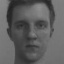
\includegraphics[width=2cm]{face_1.jpg}
		}
		\qquad
		\begin{minipage}{2cm}
			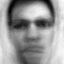
\includegraphics[width=2cm]{100.jpg}
		\end{minipage}
		\begin{minipage}{2cm}
			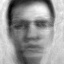
\includegraphics[width=2cm]{200.jpg}
		\end{minipage}
		\begin{minipage}{2cm}
			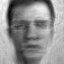
\includegraphics[width=2cm]{300.jpg}
		\end{minipage}
		\begin{minipage}{2cm}
			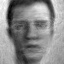
\includegraphics[width=2cm]{400.jpg}
		\end{minipage}
	\caption{Porównanie rekonstrukcji twarzy na postawie różnej liczby wykorzystanych składowych.\\ Po lewej oryginalne zdjęcie, potem kolejno rekonstrukcja z wykorzystaniem 100, 200, 300 i 400 składowych.}
	\label{fig:rekonstrukcja}
\end{figure}

Jak widać na rys. \ref{fig:rekonstrukcja} wraz ze zwiększeniem się ilości składowych jakość rekosntrukcji zdjęcia się polepsza. Użycie większej ilości składowych nie ma sensu, co można zaobserwować w wyglądzie rekonstrukcji z wykorzystanie 300 i 400 składowych. PCA jest bardzo lubianą metodą, ponieważ jest bardzo intuicyjna oraz pozwala na wizualne sprawdzenie własnych rezultatów.

W omawianym zagadnieniu wektory własne zyskały specjalną nazwę eigenfaces (twarze własne). Można zobaczyć jak wyglądają aplikując technikę odtwarzania zdjęcia na podstawie współrzędnych z przestrni o zredukowanej wymiarowości. Efekty zostały zaprezentowane na rys. \ref{fig:eigenfaces}. 

Jak można łatwo zaobserwować wektory 0-4 zawierają najbardziej istotne zmiany pomiędzy poszczególnymi obrazami ze zbioru obserwacji. Wektora 392-396 przypominają losowy szum i niosą informację o szczegółach twarzy. Można zauważyć że pominięcie składowych z niższą wartością własną powoduje mniejszą utratę informacji.


\begin{figure}
\centering
	\parbox{2cm}{
		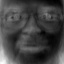
\includegraphics[width=2cm]{0.jpg}
		}
	\begin{minipage}{2cm}
		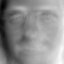
\includegraphics[width=2cm]{1.jpg}
	\end{minipage}
	\begin{minipage}{2cm}
		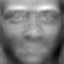
\includegraphics[width=2cm]{2.jpg}
	\end{minipage}
	\begin{minipage}{2cm}
		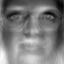
\includegraphics[width=2cm]{3.jpg}
	\end{minipage}
	\begin{minipage}{2cm}
		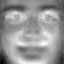
\includegraphics[width=2cm]{4.jpg}
	\end{minipage}\\
	
	\begin{minipage}{2cm}
		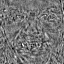
\includegraphics[width=2cm]{392.jpg}
	\end{minipage}
	\begin{minipage}{2cm}
		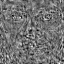
\includegraphics[width=2cm]{393.jpg}
	\end{minipage}
	\begin{minipage}{2cm}
		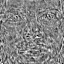
\includegraphics[width=2cm]{394.jpg}
	\end{minipage}
	\begin{minipage}{2cm}
		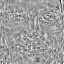
\includegraphics[width=2cm]{395.jpg}
	\end{minipage}
	\begin{minipage}{2cm}
		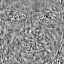
\includegraphics[width=2cm]{396.jpg}
	\end{minipage}
	
	\caption{Porównanie eigenfaces. \\ Górny wiersz - wektory 0-4, dolny wiersz - wektory 392-396.}
	\label{fig:eigenfaces}
\end{figure}








\subsubsection{PCA jako samodzielny system rozpoznawania twarzy}
Principle komponents analysis powoduje przeniesienie zdjęcia mającego wizualną reprezentację na abstrakcyjny wektor liczb. Umożliwia to skontruowanie klasyfikatora z wykorzystaniem algorytmów umożliwiających klasyfikację. Jest to zagadnienie dobrze znane w dziedzinie Pattern Recognition (rozpoznawania wzorców) i opracowano wiele rozwiązań tego problemu. Zastosowanie algorytmów typu k-NN (k Nearest Neighbour - k najbliższych sąsiadów) lub NM (Nearest Mean - najbliższy średnia) umożliwia zaklasyfikowanie danego algorytmu do jednej z grup. Jest to możliwie dzięki wykorzystaniu reprezentacji zdjęcia jako wektora liczb. Oba algorytmy dysponują zbiorem uczącym, który opisuje dane grupy do których może zostać klasyfikowany dany wzorzec. 
W przypadku NM dla każdej z grup obliczana jest średnia wektorów, następnie obliczana jest odległość między wektorem podlegającym klasyfikacji, a średnimi zbiorów. Wektor zostaje zaklasyfikowany do zbioru, którego średnia jest w najmniejszej odległości od wektora. 
W przypadku algorytmu k-NN odległość jest obliczana pomiędzy wszystkimi wektorami ze zbioru uczącego. Następnie zostaje wybrane k najbliższych sąsiadów. Zbiór, którego najwięcej przedstawicieli zostało wybranch wygrywa. Dla przypadku dychotomii jeżeli k jest nieparzyste możliwa jest jednoznaczna klasyfikacja. Gdy ilość zbiorów do których można zaklasyfikować obraz jest większa od dwóch możliwe jest wystąpienie wypadku w którym nie można jednoznacznie zaklasyfikować obiekt. 
W przypadku systemu kontroli dostępu może być rozsądne wprowadzenie maksymalnej odległości między średnią lub najbliższym sąsiadem a klasyfikowanym wektorem przy której może następić klasyfikacja. Powyżej tej odległości obraz nie powinien być zaklasyfikowany do którejkolwiek z grup. 
Dodatkowo warto zwrócić uwagę na brak kontroli PCA nad przetwarzanymi danymi. Jest to metoda statystyczna, na jej wejście można podać zdjęcie myszy lub samochodu, które zostanie przetworzone. Nie wiadomo jakie współrzędne można uzyskać, dzięki takiej operacji. System rozpoznawania twarzy powinien więc odrzucić takie zdjęcie na etapie wykrywania pozycji twarzy.
 
 
\section{Zebranie zbioru danych uczących}
\subsection{Metodyka}

Ile obrazów było w zbiorze uczącym dla PCA

Badanie wpływu oświetlenia
Badanie wpływu kątu pod jakim zrobiono zdjęcie
Badanie wpływu okularów?
Badanie wpływu podania randomowego zdjęcia na system (np. zdjęcie mojego biurka)


\subsection{Automatyzacja badań}


\section{Zakończenie}

\newpage
\begin{thebibliography}{9}

\bibitem{Pattern recognition}
Christopher M. Bishop.
\textit{Pattern recognition and machine learning}.
Springer Science + Business Media, New York 2009

\bibitem{Osowski}
Stanisław Osowski.
\textit{Sieci Neuronowe w ujęciu algorytmicznym}
Wydawnictwo Naukowo-Techniczne, Warszawa 1996

\end{thebibliography}

\end{document}